% -*- TeX -*- -*- UK -*- -*- Soft -*-

\chapter{playground.tensorflow.org}
\label{sec:playground.tensorflow.org}

\section{Introduction}

Google created \lstinline{playground.tensorflow.org}
\cite{GooglePlayground2019} as a safe learning environment where you can experiment with neural nets and deep learning without writing code.  This is a convenient way to become acquainted with \ac{ML}.

On opening the website has the following graphical interface display: 
 
\begin{figure*}[h]
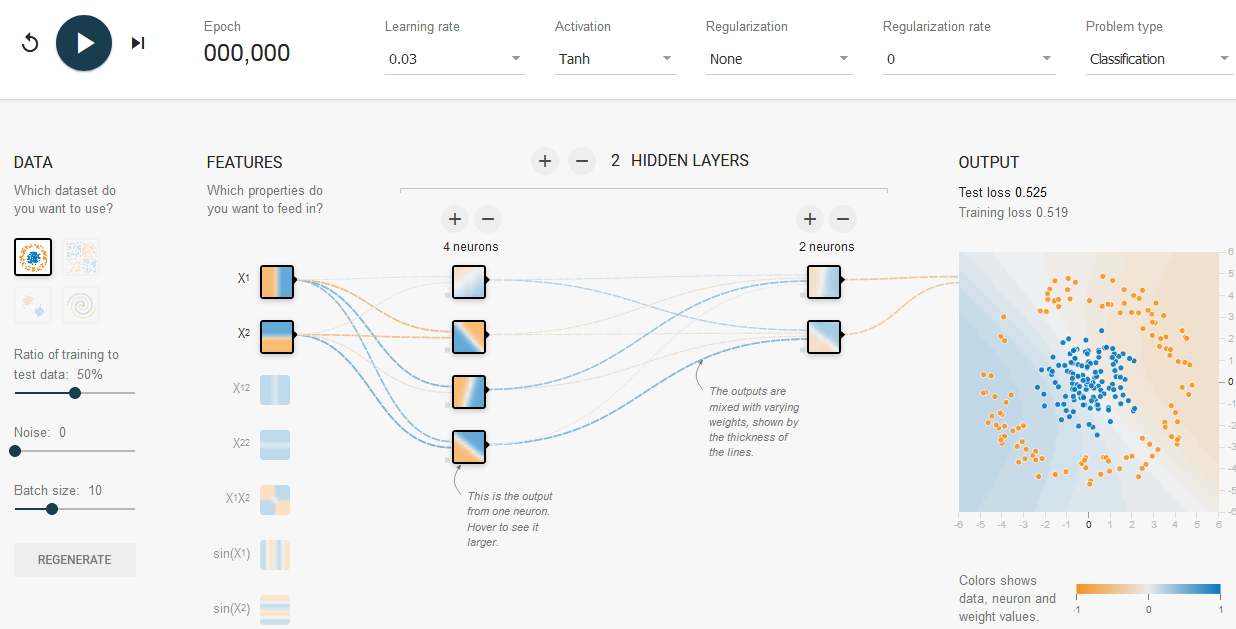
\includegraphics[width=\textwidth]{playground01}
\end{figure*}

Essentially the site provides a neural net training environment where you can select a number of different elements of the project: you can 
(1) select different \ac{2-D} data sets on the left, 
(2) set learning parameters on the left,
(3) specify how features  should be extracted from the data set,
(4) change the number of layers and/or neurons in each layer,
(5) see the output from the net, showing the classification performance.
Along the top you can select learning rate, the activation function, regularisation, and the type of problem. 

Keep the original inputs with two hidden layers and press the run button. 

\begin{figure*}[h]
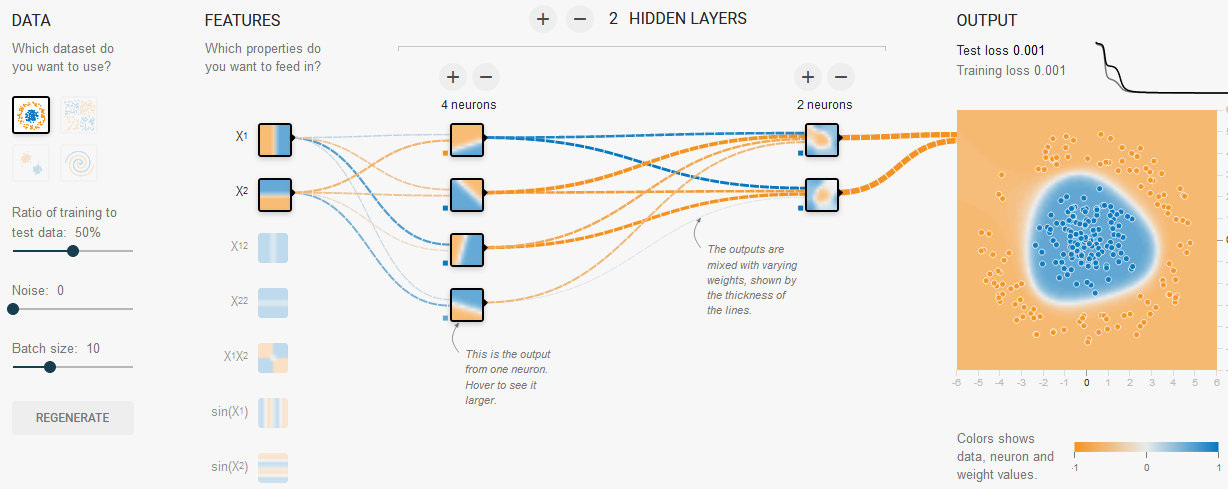
\includegraphics[width=\textwidth]{playground02}
\end{figure*}
\FloatBarrier

Observe how the net trains. After a while it classifies perfectly.  Move the mouse over the neurons to observe the single neuron's contribution to the classification in the larger image on the right (this is the effect that the neuron has in the network). Hover over the lines and observe that the thickens of the lines describes the weight of the connection. If you click on the line you can change the weight and immediately see the effect in the output. 

Next change the network design by changing the number of layers and neurons. Evidently the problem can be solved with a single hidden layer with three neurons.

\begin{figure*}[h]
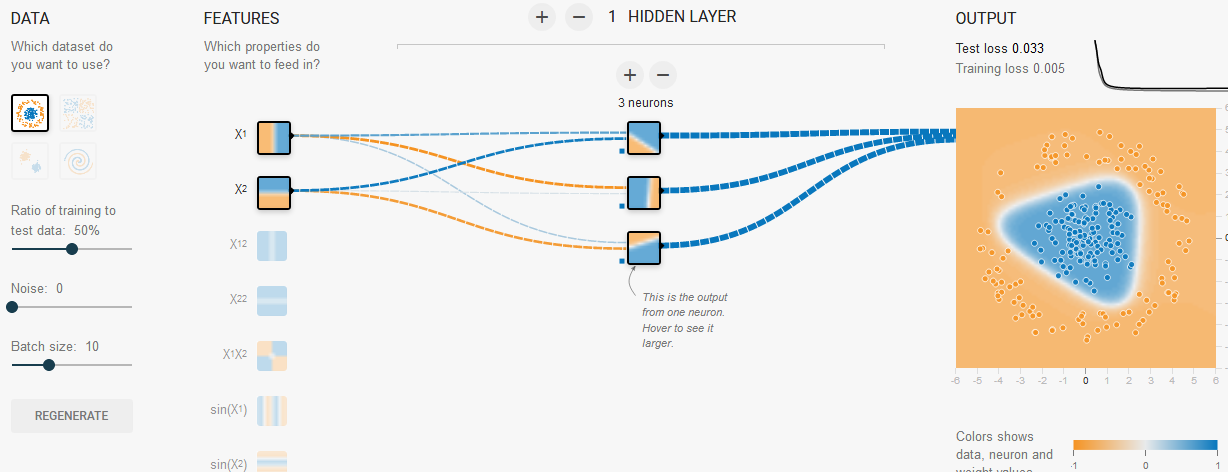
\includegraphics[width=\textwidth]{playground03}
\end{figure*}

\FloatBarrier

Select a new data set and give it two hidden layers and a few more neurons. Observe that in the following case, most of the work is done in the first hidden layer by the first and third neurons, see their weight compared to the other neurons' weights.

\begin{figure*}[h]
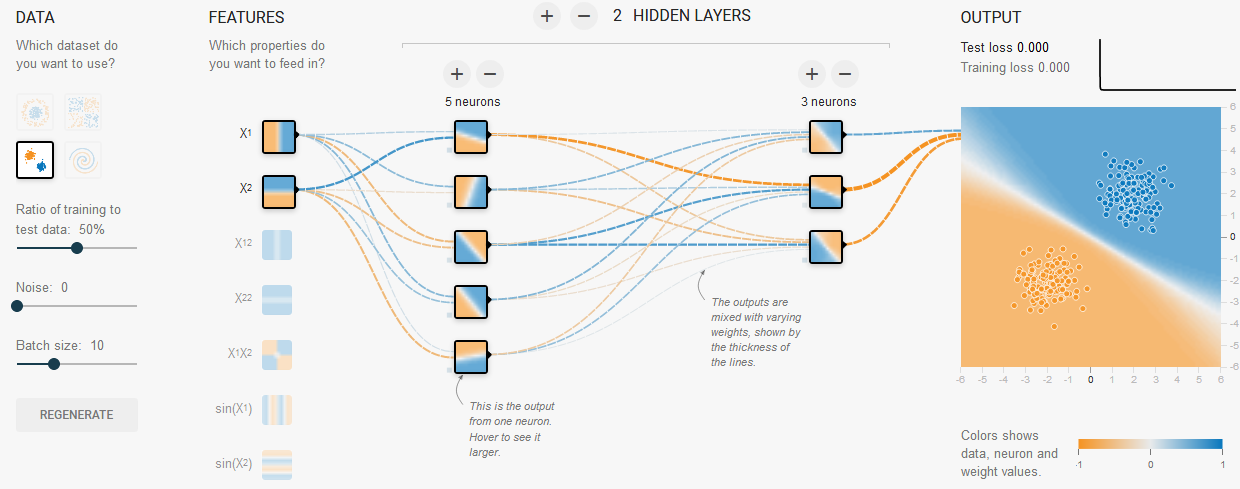
\includegraphics[width=\textwidth]{playground04}
\end{figure*}

\FloatBarrier

Reduce the number of neurons in the first hidden row to two and observe that the classification is equally good.  Next remove the second hidden layer and observe that the classifier still performs well. What we have here is a simple straight line classifier.

Next, select the spiral data set and add two more hidden layers and many more neurons.  Also select the ReLu activation function in the top row.  See how nicely the classifier creates the boundaries to discriminate between the two classes!  Note that the top neuron in the third hidden layer has no weight feeding into the output, it can safely be removed.

\begin{figure*}[h]
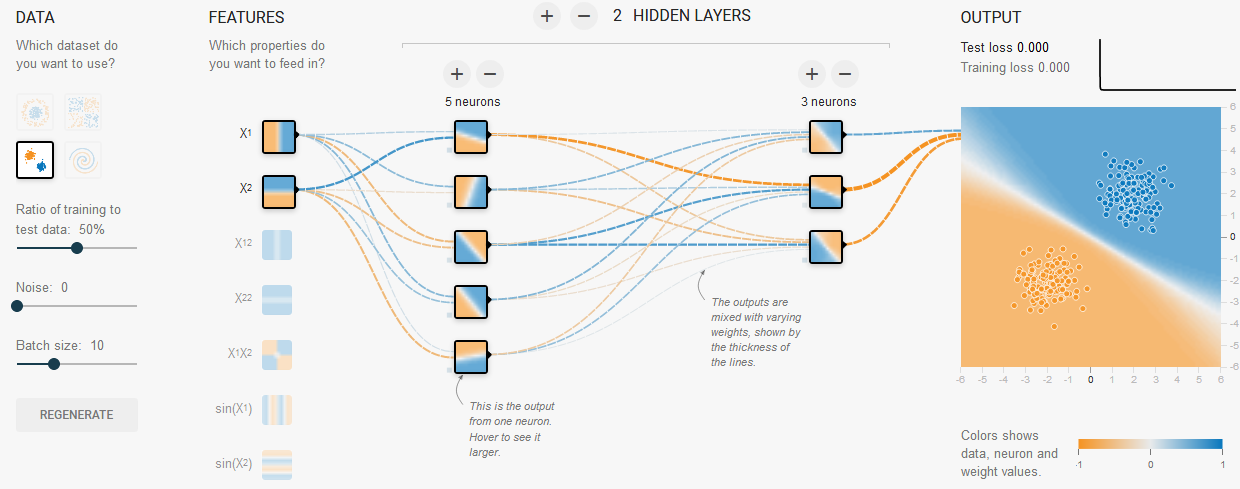
\includegraphics[width=\textwidth]{playground04}
\end{figure*}

\FloatBarrier

This tool is hardly sufficient to develop ant real world practical solution, but it does provide a very nice play pen to develop an understanding of at least the underlying principles.
